% CCN 2027 Extended Abstract draft (mechanism-first adaptation).
% Format target: 2 pages of text, tables, and figures (title block and abstract included);
% references may extend onto additional pages; no appendix or supplement allowed.
% Template: ccn.cls from github.com/cogcompneuro/ccn-template (2026 release); update to the
% 2027 template when CCN posts it.
\documentclass{ccn}

\addbibresource{references.bib}

\newcommand{\contrast}{C_{\mathrm{att-acc}}}

\title{Readable but Unused: Decodable Intent Does Not Control\\Moral Judgment in Language Models}

\author{Anonymous}

\begin{document}

\maketitle

\begin{abstract}
Language models pass explicit false-belief tests, but do they use mental-state information downstream?
Using a belief $\times$ outcome moral-judgment factorial from cognitive neuroscience, we found that six open instruct models answered 82--99\% of hard false-belief items correctly while condemning accidents more than failed attempts, the reverse of the adult pattern.
In eight open checkpoints, intent was linearly decodable from hidden states, but neither item-level decodability nor representational geometry tracked behavior, and adding the intent direction barely changed ratings while an outcome direction changed them substantially.
Erasing a linear outcome component made judgments more intent-sensitive in two of three models.
Outcome information decodable before the outcome sentence was carried by a foreshadowing sentence, and deleting that sentence reduced outcome decoding to chance.
Representing mental-state information and using it in judgment can dissociate.
\end{abstract}

\begin{figure*}[t]
  \centering
  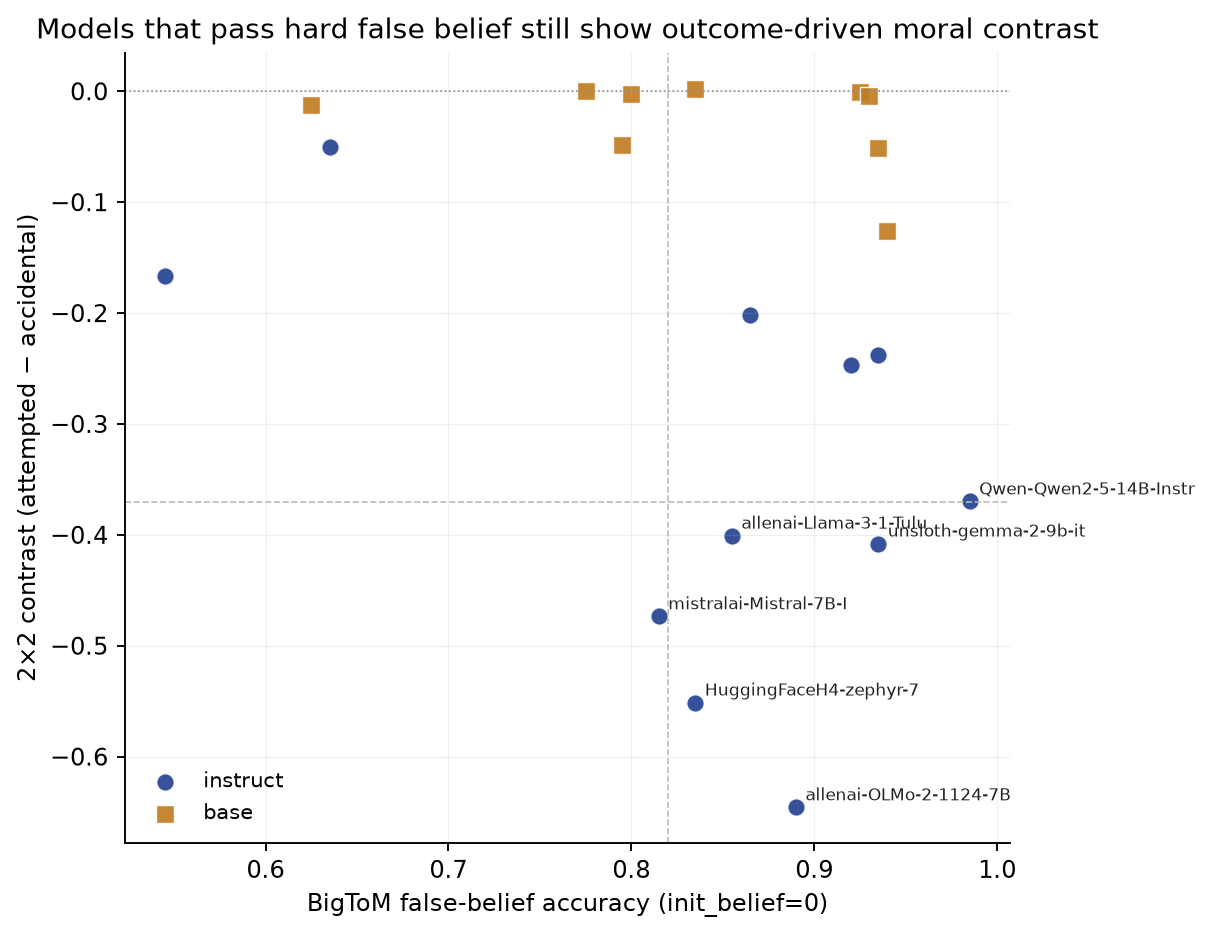
\includegraphics[width=0.40\textwidth]{figures/tom_vs_contrast.png}\hfill
  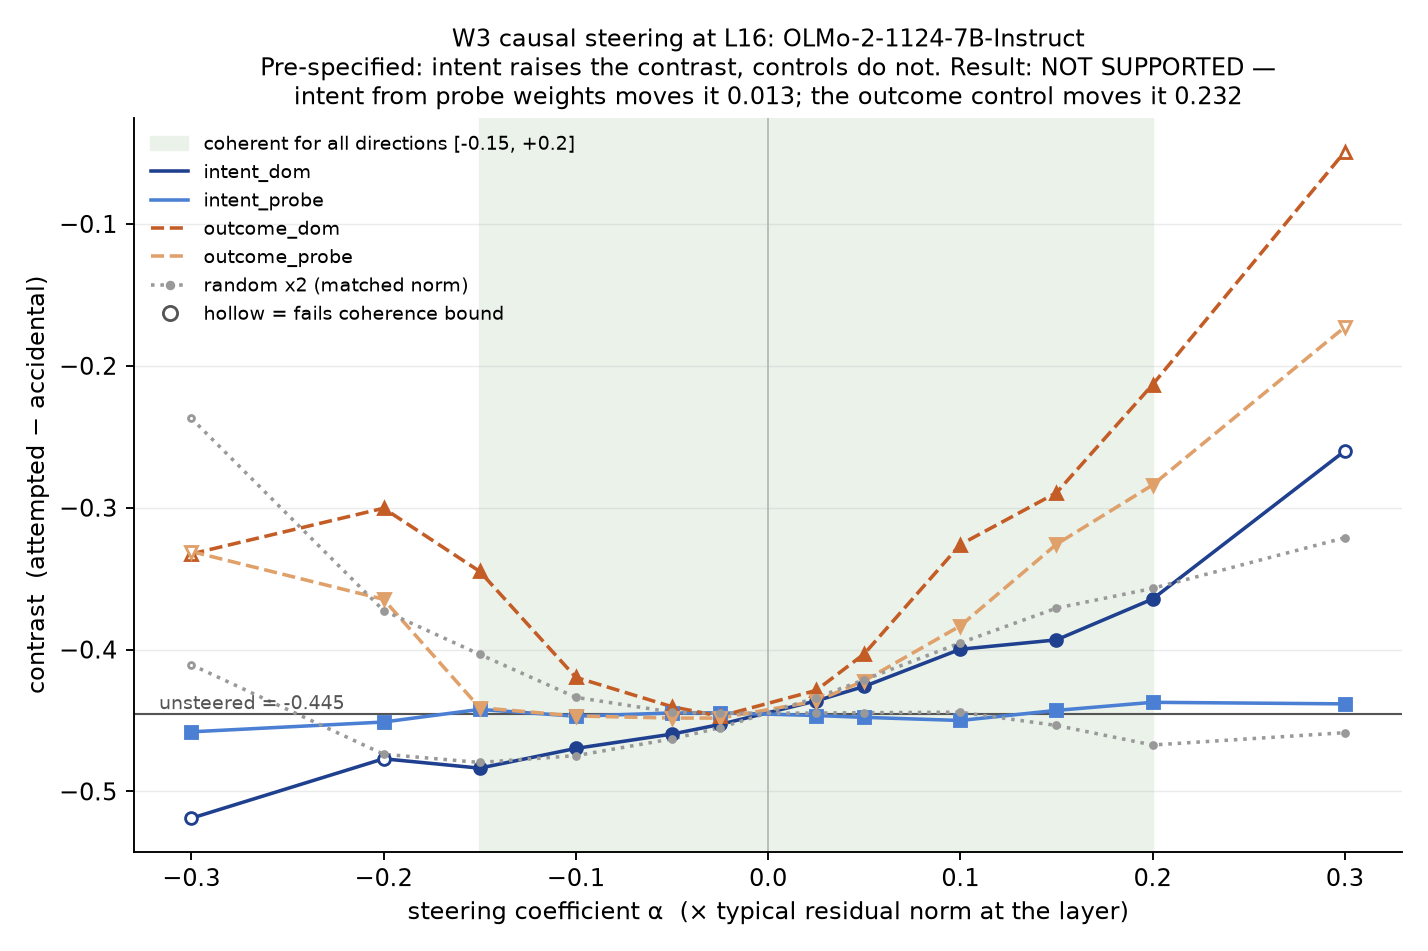
\includegraphics[width=0.56\textwidth]{figures/w3_steering_OLMo.png}
  \caption{\textbf{Left:} Hard false-belief accuracy versus attempted-minus-accidental contrast for open models (blue = instruct, ochre = base); engaged instruct models pass false belief yet keep negative contrasts.
  \textbf{Right:} Adding hidden-state directions at layer 16 of OLMo-2-7B-Instruct. The probe-weight intent direction barely moves the contrast within the coherent range (shaded); outcome directions move it substantially; gray = matched random directions.}
  \label{fig:main}
\end{figure*}

\section{Introduction}

Explicit ToM benchmarks report strong model performance \citep{gandhi2023bigtom,strachan2024testing}, yet small perturbations can remove it \citep{ullman2023alterations}, and explicit inference can fail to transfer to applied judgment \citep{gu2026simpletom}.
Belief information is also linearly decodable from activations \citep{zhu2024beliefs}.
We ask whether decodable intent \emph{controls} a downstream judgment.
The belief $\times$ outcome paradigm \citep{young2007neural,young2008belief} crosses benign or harmful intent with benign or harmful outcome; adults condemn failed attempts far more than accidents (contrast $\contrast=+0.666$), whereas children and some societies weight outcomes more \citep{cushman2013development,barrett2016societies}, so human values serve as descriptive references only.

\section{Methods}

We used 298 vignettes from published appendices \citep{young2008belief,young2009innocent,young2011ignorance}, merged into 53 independent scenario groups after removing reprints and an outcome-leaking text artifact.
Twenty open models were scored as the expected value over rating-digit probabilities; $\contrast$ is attempted minus accidental condemnation.
For eight OLMo-2 and Qwen2.5 checkpoints, logistic probes decoded intent and outcome from the residual stream under leave-scenario-group-out folds, at the final token and the end of the belief clause.
We linked decodability to behavior at the item level and with RSA across model pairs \citep{kriegeskorte2008rsa}; added intent, outcome, and matched random directions to the residual stream in two models; and applied rank-one LEACE outcome erasure \citep{belrose2023leace} in three models, pre-registering \emph{recovery} (contrast moves while $\geq$50\% of four-cell spread is retained) versus \emph{collapse}.
Follow-up probes with within-scenario permutation nulls decoded outcome at the belief endpoint with and without the foreshadowing sentence, and both factors at 40 story positions in three base/instruct pairs.

\section{Results}

\textbf{Stating versus using.}
None of 20 open models placed attempted above accidental harm (14 reversed, six tied).
The six engaged instruct models scored 0.815--0.985 on hard BigToM while producing contrasts of $-0.370$ to $-0.646$ (Fig.~\ref{fig:main}, left).
In three public pipelines, supervised fine-tuning alone moved the contrast negative.

\textbf{Decodable but not predictive.}
At the belief-clause endpoint, intent decoding reached 0.90--0.98 (span-matched lexical baseline 0.591).
Item-level intent margins did not predict contrast (slope $+0.062$, 95\% CI $[-0.146,+0.270]$; pre-specified meaningful slope $+0.30$), and RSA geometry--behavior correspondence across 28 model pairs was $r=+0.098$ $[-0.31,+0.46]$.
Outcome was also decodable at the belief endpoint (0.70--0.87 across 14 checkpoints; word TF--IDF baseline 0.631), but the foreshadowing sentence is the only earlier text that differs between outcome partners; deleting it reduced outcome decoding to chance (0.496--0.504 in all six models tested), so early outcome decodability is a readout of stated text, not prediction.
Token-wise, intent rose to 0.95--0.98 at the end of the belief clause and declined by 0.16--0.21 over later bins; base and instruct curves were nearly indistinguishable, although their behavioral contrasts differed by $-0.18$ to $-0.69$.

\textbf{Readable but not controlling.}
At coherent doses, the probe-weight intent direction changed $\contrast$ by at most 0.013 (OLMo) and 0.016 (Qwen), versus 0.232 and 0.259 for outcome directions (Fig.~\ref{fig:main}, right), even though intent steering drove held-out intent decoding from about 0.89 to 0.50.
Outcome erasure produced recovery in OLMo ($+0.318$; 51\% spread retained) and Qwen ($+0.231$; 67\%) but collapse in Tulu ($+0.348$; 38\%).
A scenario-perturbation control failed in Qwen while orthogonalized nuisance erasures were inert, so outcome is the most effective direction tested, not an established unique mechanism.

\textbf{Development.}
Across 26 Pythia-1.4B and 20 OLMo-2-7B pretraining checkpoints, intent and outcome structure in representational geometry developed smoothly and depended on read position, while no pretraining checkpoint produced gradeable ratings; in OLMo the first gradeable point was SFT.

\section{Discussion}

In the open models tested, intent is linearly readable and internally manipulable, yet the graded moral readout depends mainly on outcome structure.
This dissociation argues for evaluating machine ToM at separate levels: explicit inference, applied behavior, and representation--behavior links with controlled interventions.
Claims are bounded to open models up to 14B parameters and to linear, single-layer interventions; human references are not item-matched; and behavior-only reruns of nine closed-API models were heterogeneous (four of nine placed attempts above accidents), so no universal claim about current models is made.

\section*{Acknowledgments}
Portions of this abstract were drafted with an AI writing assistant from the authors' project results; authors must describe this use and verify all content before submission.

\printbibliography

\end{document}
